\section{Overview: The Building Adapter}
In this work, we adopt a transfer learning based approach proposed in \cite{lwe} to learn a set of statistical classification models based on features extracted from sensor stream readings from
one building, and transfer the learned models to label sensors in another building.
% The approach presented in~\cite{lwe} uses a suite of base classifiers and leverges the consistency between classifier and cluster structure to weigh the results of each classifier.
% We make several changes to the original algorithm to address the specific challenges we face:
% 1) both the data and the names of streams are used in our approach: an
% ensemble of base learners are constructed with data features and applied to the target building, while the
% cluster structure on the name features in the target building guides the decision process about how to weigh each classifier;
% 2) we customize the weight estimation algorithm to improve its performance in our setting;
% and 3) to handle variations in point names, we use a non-parametric Bayesian approach to identify cluster structure.
Based on the insight that the data and the names of sensors characterize different properties of a sensor point, our algorithm exploits features extracted from both the data and the point names to accomplish the transfer.
%We also define new weighting function for base classifiers considering our specific problem setting.
In the rest of the section, we first elaborate how to construct those two different types of features and then concentrate on the proposed transfer learning method.

\subsection{Feature Representation}\label{feature}
Our transfer learning based approach exploits two common attributes of the sensor points in a building - the actual data readings and the text string-based point names, both of which play an important role for differentiating sensor types.
In this section, we describe the construction of two different sets of feature vectors, i.e., data features and name features.

\begin{figure*}[ht!]
\centering
  \begin{subfigure}{0.32\textwidth}
                \centering
    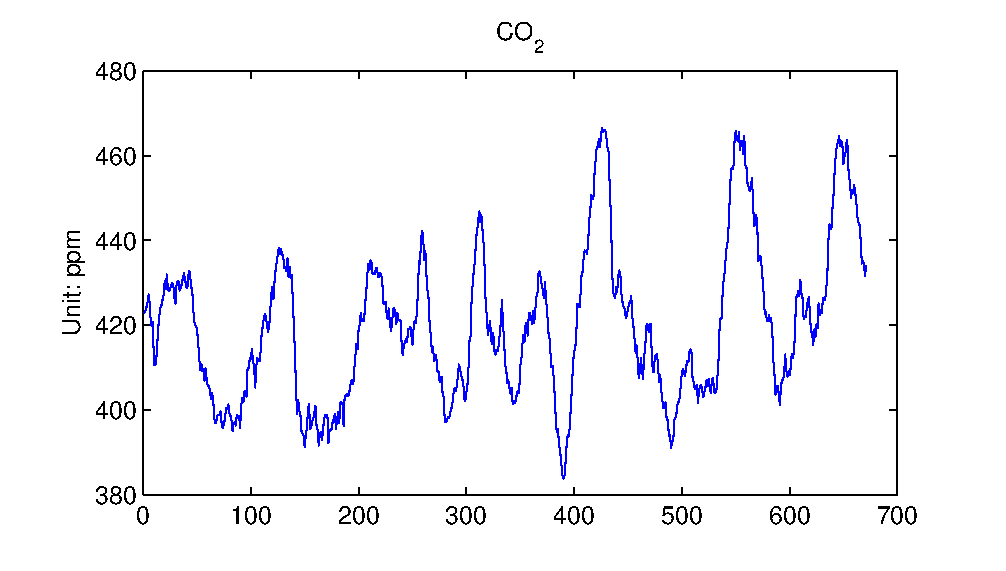
\includegraphics[width=\textwidth]{./fig/co2.eps}
                \caption{$CO_{2}$}
  \end{subfigure}
  \begin{subfigure}{0.32\textwidth}
                \centering
    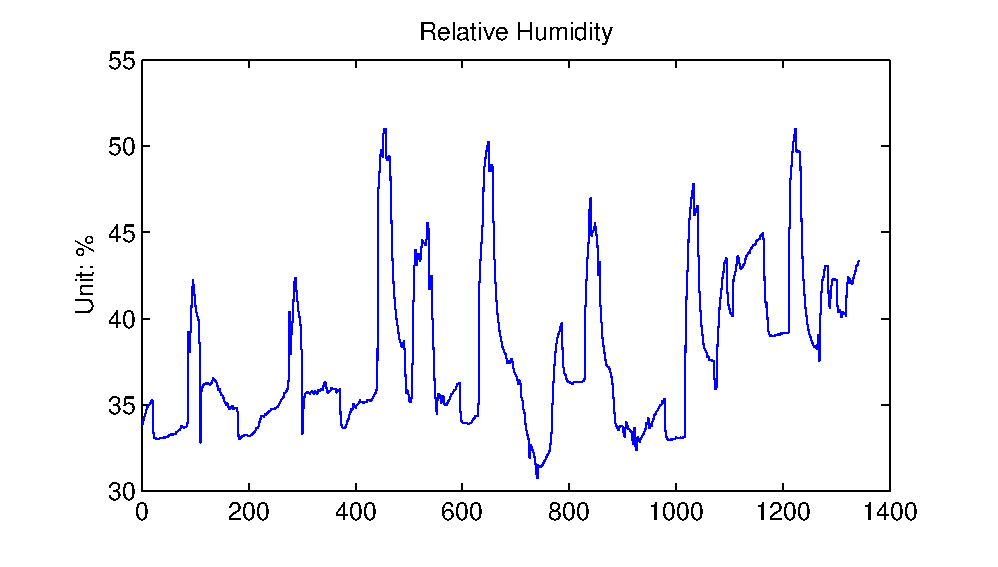
\includegraphics[width=\textwidth]{./fig/rh.eps}
                \caption{Humidity}
  \end{subfigure}
  \begin{subfigure}{0.32\textwidth}
                \centering
    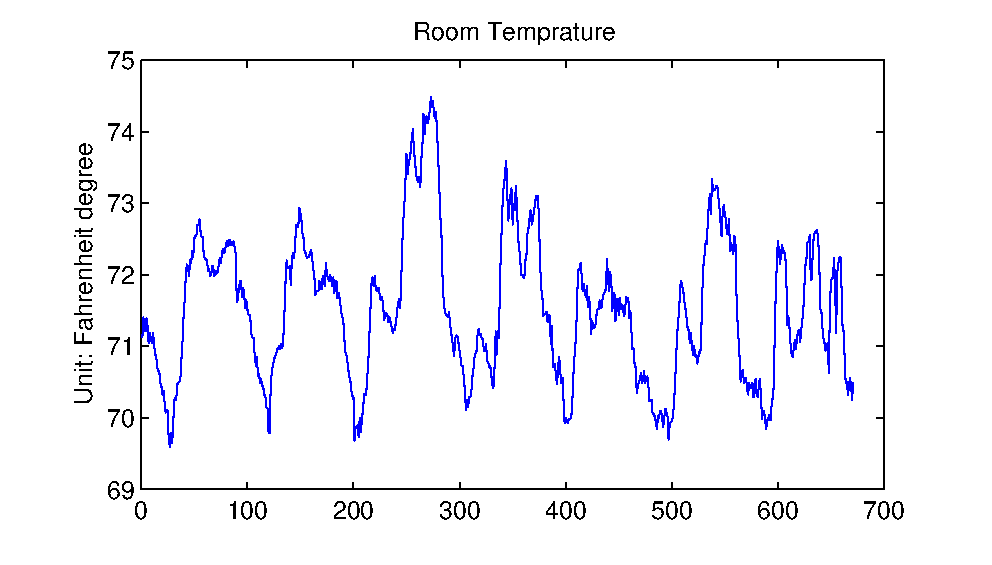
\includegraphics[width=\textwidth]{./fig/rmt.eps}
                \caption{Room Temperature}
  \end{subfigure}
  %row2
  \begin{subfigure}{0.32\textwidth}
                \centering
    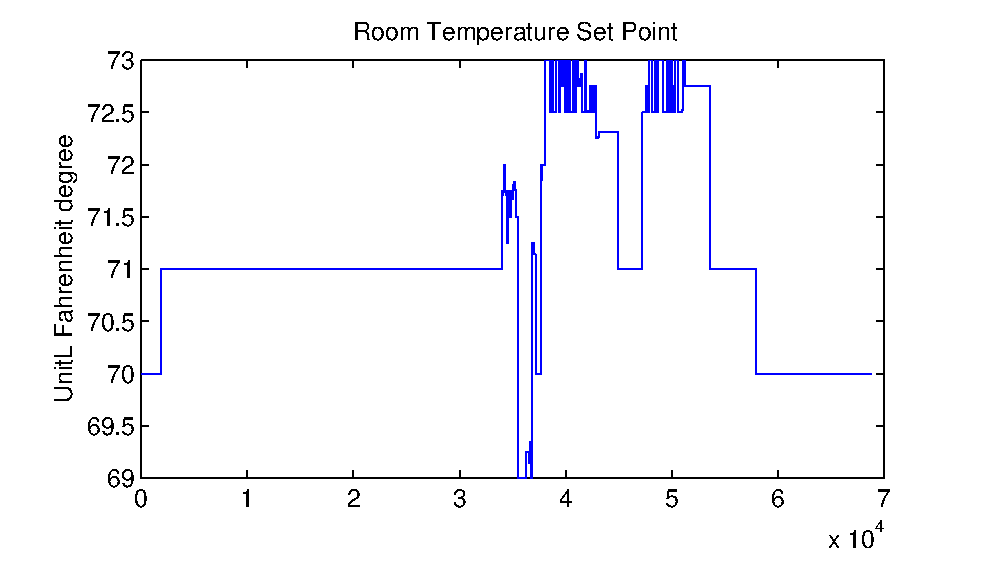
\includegraphics[width=\textwidth]{./fig/stpt.eps}
                \caption{Room Temperature Set Point}
  \end{subfigure}
  \begin{subfigure}{0.32\textwidth}
                \centering
    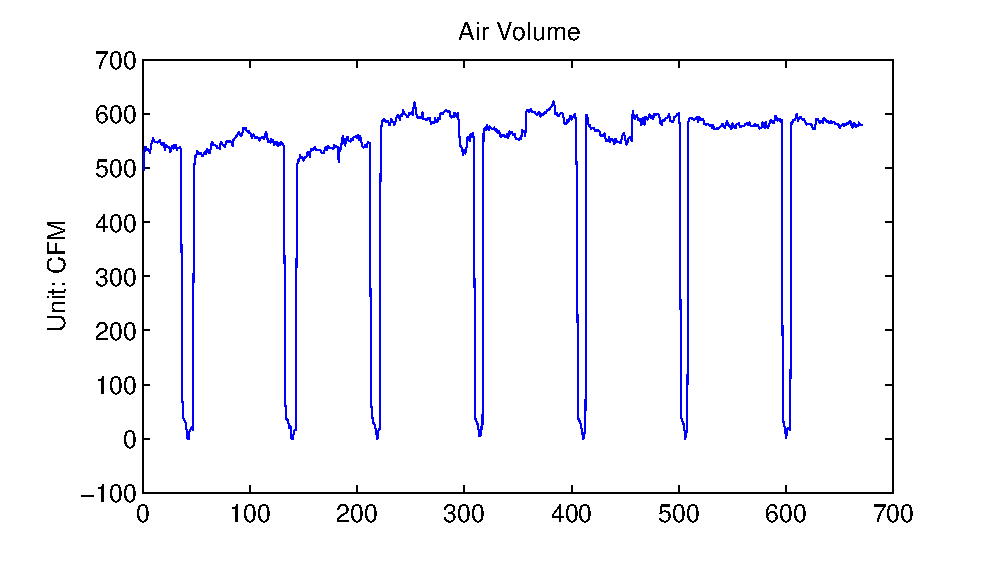
\includegraphics[width=\textwidth]{./fig/vav.eps}
                \caption{VAV Air Volume}
  \end{subfigure}
  \begin{subfigure}{0.32\textwidth}
                \centering
    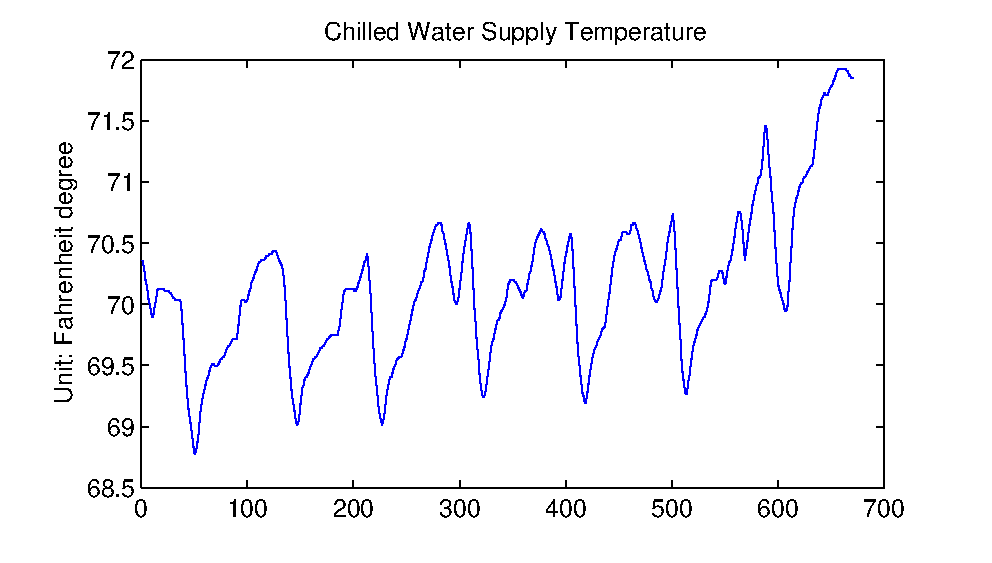
\includegraphics[width=\textwidth]{./fig/cwt.eps}
                \caption{Chilled Water Supply Temperature}
  \end{subfigure}
%\caption{Different types of sensors occupy different amplitude bins in the time domain with different short term dynamics.}
\caption{Different types of sensor generally have different amplitudes that can be separated and binned to characterize the data.}
\label{fig:example}
\end{figure*}

\subsubsection{Data Features}
A signal\footnote{In this paper, we use the term ``signal'', ``trace'' and ``time series'' \textit{interchangeably}.} in the time domain is a trend of sensor reading.
Different types of sensors generally have different amplitudes that can be separated and binned,
as demonstrated in Figure~\ref{fig:example}.
Similar to piecewise aggregated approximation (PAA~\cite{paa}) -- where the mean is calculated in a fixed-length window --
we compress the signal by computing a set of summary statistics over fixed-length windows.
Table~\ref{table:fd} shows a summary of the statistics we calculate as data features.


\begin{table}[h]
\centering
\begin{tabular}{r|l|l}
\hline
Category                   & Statistical Function & \multicolumn{1}{l}{Acronym} \\ \hline\hline
\multirow{2}{*}{Extrema}   & Minimum                 & min                          \\ \cline{3-3}
                           & Maximum                 & max                          \\ \hline
\multirow{2}{*}{Average}   & Median                  & emd                          \\ \cline{3-3}
                           & Root Mean Square        & rms                          \\ \hline
\multirow{2}{*}{Quartiles} & 1st and 3rd Quartiles   & 1q, 3q                       \\ \cline{3-3}
                           & Inter-quartile range    & iqr                          \\ \hline
\multirow{3}{*}{Moments}   & Variance                & var                          \\ \cline{3-3}
                           & Skewness                & skew                         \\ \cline{3-3}
                           & Kurtosis                & kurt                         \\ \hline
Shape                      & Linear Regression Slope & slope                        \\ \hline
\end{tabular}
\caption{Statistical features extracted in window level for each time series data.}
\label{table:fd}
\end{table}

Our feature extraction process consists of three steps.
First, each sensor trace is segmented into N hour-long windows with 50\% overlap between consecutive windows. Second, for each time window, we compute the statistics shown above.
%This produces a vector where each component is a a %statistic over the window. %slides over the entire trace, such as
For example, the vector for $MIN$ is computed as follows:
$MIN = \{min^{1}, min^{2}, ..., min^{N}\}$, where N is the number of time windows. We compute a similar vector for each statistic show in the table.
%Each vector, reflects short term changes that are useful for classification.
Third, we compute a statistical summary of these vectors. For each vector we compute the minimum, maximum, median and variance, resulting in a feature
vector containing 44 variables:
\begin{displaymath}
\begin{split}
F = \{min(MIN), max(MIN), \\
median(MIN), var(MIN),\\
...\\
min(SLOPE), max(SLOPE), \\
median(SLOPE), var(SLOPE)\}
\end{split}
\end{displaymath}
$F$ is the data feature vector for each sensor trace used in our study.


\subsubsection{Name Features}
Sensor point names are short text strings with several concatenated abbreviations, as shown in Table~\ref{table:ex}.
To extract features from a point name, we convert all alphabetical characters to lower cases and trim out numerical characters.
For example, \texttt{Zone Temp 2 RMI204} becomes \texttt{\{zone, temp, rmi\}}.
%To capture possible variants of abbreviations in point names, e.g., ``tmp'' and ``temp'' for temperature, we adopt $k$-mers \cite{leslie2004mismatch} as our features.
We use $k$-mers \cite{leslie2004mismatch} to capture variations in type abbreviations, e.g., ``tmp'' and ``temp'' for temperature.
The term $k$-mer refers to all the possible substrings of length $k$ in a given string. This feature is often used in protein and gene sequence analysis and
it helps measure sequence similarity without requiring alignment.

We limit the k-mers computation within a word boundary.
In general, smller $k$ will increase the overlapping between generated k-mers, making points less differentiable.
Therefore, we compute all k-mers of length 3 and 4 for each point name.
For example, \texttt{\{zone, temp, rmi\}} yields a set of k-mers \texttt{\{zon, one, tem, emp, rmi\}} when $k$=3.
A dictionary of k-mers is constructed with all the k-mers generated from each point name.
Each point name is converted into a feature vector based on the frequency of k-mers in it.
For example, a set of k-mers \texttt{\{zon, tem, emp, zon\}} will be transformed to a vector
\texttt{(2,0,1,1,0)} with the dictionary \texttt{\{zon, one, tem, emp, rmi\}}, meaning \texttt{zon} occurs twice, \texttt{one} does
not appear, and so forth.
This feature representation of point names will be used for examining classification performance.

%\subsection{Transfer Learning for Cross-Building Sensor Type Classification}
%The use of transfer learning is motivated by the fact that people often have one or only a few buildings labeled of which they want to take advantage to aid the labeling of a new buidling.
%Transfer learning is a useful technique in the building space because the effort it takes to label sensors in a single building is high.
%We want to leverage the knowledge gained in one building to quickly label another with minimal effort.
%One category of transfer learning uses well-labeled data from one domain\footnote{A ``domain'' particularly refers to a data set in this paper.}
%to classify examples in a new, related domain.
%We assume we have well-labeled training set examples but do not have any labeled examples from the testing set.
%Such knowledge transfer is possible when the training domain and the test domain have the same set of class labels.
%Classical supervised learning techniques are not useful for transferring knowledge across domains in this setting because
%The reason that traditional supervised learning techniques is not successful in transferring knowledge across domains in our case is because
%it requires the training and testing examples to be sampled i.i.d. from the same distribution. This basic requirement does not hold here.

%For example, the classiers can be trained from several relevant domains or built using different learning algorithms on the same domain.


\subsection{Locally Weighted Ensembles}

To encapsulate the information from one labeled building and transfer it across
buildings, we construct a few classifiers with different learning algorithms,
using the same set of data features from the source building\footnote{the
  building we learn from is the ``source'', all others are ``targets''}.  Each
classifier contains a different ``perspective'' for that building, due to the
inductive bias of the underlying model.  We refer to these classifiers as {\it
  base} models\footnote{We use the term ``model'' and ``classifier'' {\it
    interchangeably} in this paper.} and combine them for type classification in the
target building.  

Specifically, the instance-based local weighting for each classifier is guided by the consistency between a classifier's predictions and the instance's local structure that is approximated by clustering; classifiers with higher consistency would be assigned a larger weight. 
Based on our previous observations, data features are more likely to transfer across buildings, thereby better for classifier construction, while name features tend to better align with the true labels therefore are more suitable for discovering unsupervised neighborhood with clustering.
We will next elaborate the intuition and detail behind employing instance-based local weighting and choosing clustering for local structure approximation.
Finally, we describe how we identify the cluster structure with a non-parametric Bayesian method.
% We will discuss the choice of data features for classifier training in the evaluation.


The performance of any particular model can vary from building to building, and different models can be effective at different regions or structures in a target building: no single model can perform well on all examples.
%Different models can be effective at different regions or structures in a target building, and
To combine the knowledge across base models,
% rather than only using any particular model, to more effectively transfer the knowledge to the new building.
% A natural choice is model averaging that additively combines the predictions of multiple base learners.
% However, the existing model averaging methods for traditional supervised learning usually assign global weights to models, which are either uniform (e.g., in Bagging~\cite{bagging}) or proportional to the training accuracy (e.g., in Boosting~\cite{boosting}), or simply relying on a specific model (e.g., single model classification).
% Such global weighting schemes may not perform well in transfer learning because different testing examples may favor predictions from different base models.
% For example, when the base models carry conflicting concepts at a testing example, the optimal choice would be a model that better represents the distribution underlying the example.
we employ a locally weighted ensemble method \cite{lwe} to combine the predictions from different base classifiers.
The weight is computed per model per example based on the consistency between the base models' predictions and the local structure of the target examples.
The consistency is measured by comparing neighborhood graphs, which we will explain in the next section.
Local weights will favor models whose predicted local structure is consistent to the estimated local structure of the target examples in the testing domain.
Let $x$ be the data feature vector of an example in the new building and $y$ be its predicted class label. Given a set of $k$ base models $M_1, \dots, M_k$ and the new testing set $D_T$ represented in the data feature view, the general Bayesian model averaging rule estimates the posterior distribution of $y$ as,
\begin{equation}\label{eq_lwe}
p(y|x)=\sum_{i=1}^k p(y|x,D_T,M_i) p(M_i|D_T)
\end{equation}
where $p(y|x,D_T,M_i) = p(y|x,M_i)$ because $x \in D_T$ and $p(y|x,M_i)$ is the label for $x$ predicted by $M_i$ and $p(M_i|D_T)$ is the probability of choosing $M_i$ given the testing set $D_T$.
Since $x \in D_T$, $p(M_i|D_T)$ is equal to $p(M_i|x)$, which is the locally adjusted weight for $M_i$ and Eq.~\ref{eq_lwe} becomes,
\begin{equation}\label{eq_sum}
p(y|x)=\sum_{i=1}^k w_{x}^{M_i} p(y|x, M_i)
\end{equation}
where $w_{x}^{M_i} = p(M_i|x)$.  A model $M_i$ is expected to have a higher weight for $x$ if $M_i$'s predicted local structure for $x$ is closer to the estimated neighborhood.
We will next explain how the weight is calculated per example.

\subsubsection{Graph-based Weight Estimation}\label{sec:gwe}
% If $p(y|x)$ is known, we can estimate the weights $w_{x}^{M_i}$ for each model by minimizing the square error between its prediction and the ground truth.
% However, in practice the truth value of $p(y|x)$ for a new building is not available a priori .
% The main task becomes to properly define the similarity between classifier's predicted structure and the true structure.
% We quickly summarize the graph-based weight estimation technique presented in~\cite{lwe} and describe two adjustments we make to fit our problem.
Assuming that $p(y|x)$ does not change much in a dense area where $p(x)$ is high~\cite{cluster},
% which means the decision boundary probably exists in areas with smaller $p(x)$.
the technique in~\cite{lwe} performs clustering on the new testing set and assumes the boundaries between clusters represent areas where $p(x)$ is small.
If the clustering boundary for the region where $x$ falls, agrees with the decision boundary of $M_i$,
% we assume that $p(y|x,M_i)$ is similar to the true $p(y|x)$ around $x$, which means
a larger weight is assigned to $M_i$ at point $x$.
In other words, if the predictions made by $M_i$ on the area surrounding $x$ have greater consistency with the clustering results, $M_i$ will be assigned
a larger weight at $x$.

Based on these observations, the weight is estimated with a graph-based algorithm.
To compute the $w_{x}^{M_i}$ for $M_i$ at point $x$, we construct two neighorhood graphs:
$G_M = (V, E_M)$ and $G_C = (V, E_C)$, for classification and clustering respectively,
where each vertex is an example and $V = D_T$. In $G_M$, an edge exists between two vertices (denoting the two examples are ``neighbors'') if and only if $M_i$ predicts the same label for these two examples. Likewise, in $G_C$, an edge exists between two vertices if and only if these two examples reside in the same cluster.
If the neighbors of $x$ on both graphs significantly overlap, then $M_i$ will be assigned a larger weight.
So the weight $w_{x}^{M_i}$ for $M_i$ at $x$ is proportional to the similarity of the two graphs:
\begin{equation}\label{eq_sim}
w_{x}^{M_i} \propto s(G_M, G_C|x) = \frac {|V_M \cap V_C|} {|V_M \cup V_C|}
\end{equation}
where $V_M$ ($V_C$) is the set of neighbors of $x$ on graph $G_M$ ($G_C$), $|X|$ is the cardinality of set $X$, and $s(G_M, G_C|x)$ is the similarity between two graphs.
Figure~\ref{fig:graph} illustrates an example of neighborhood graphs for an example $x$ (in grey circle): model 1 has a similarity of 0.75 with the cluster graph
 while model 2 has a similarity of 0.5 with the cluster graph.

\begin{figure}[h]
\centering
    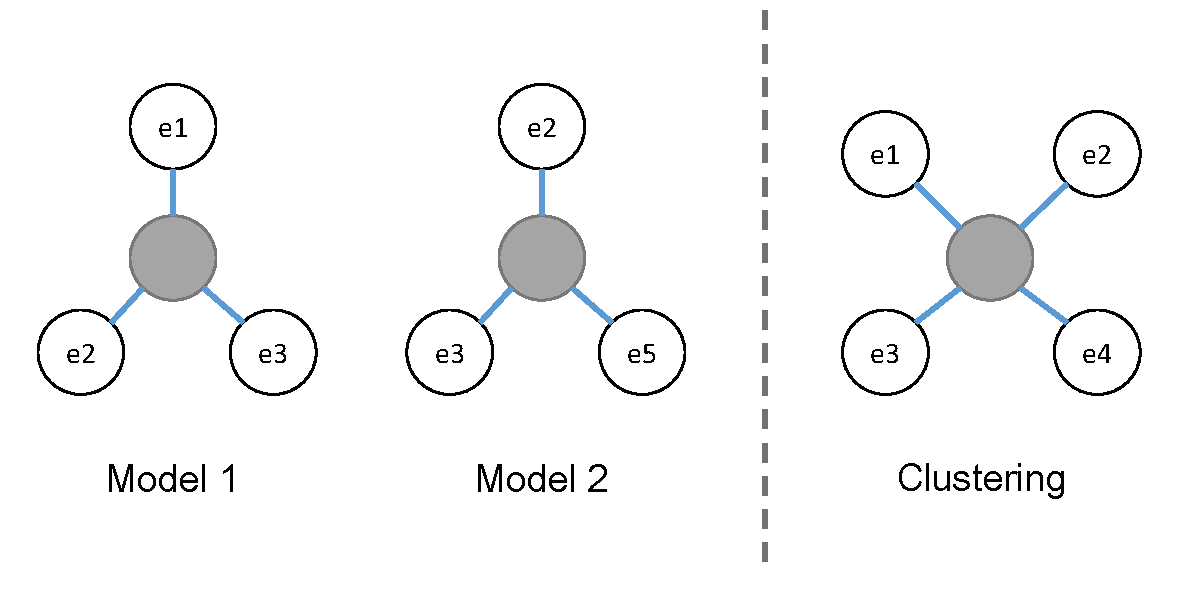
\includegraphics[width=0.4\textwidth]{./fig/lwe_graph}
\caption{An example of local neighborhood graphs of $x$ (in grey circle).}
\label{fig:graph}
\end{figure}

%With Eq.~\ref{eq_sim} defined,
The weight for each $M_i$ is calculated by normalizing among all similarity scores:
\begin{equation}\label{eq_norm}
w_{x}^{M_i} = \frac {s(G_{M_i}, G_C|x)} {\sum_{i=1}^k s(G_{M_i}, G_C|x)}
\end{equation}
The final prediction for $x$ is simply $\hat y = argmax_y \enspace p(y|x)$ as $p(y|x)$ is defined in Eq.~\ref{eq_sum}.

\paragraph{Distance-based Adjustment}
In some cases the similarity score can be problematic. Consider the case shown in Figure~\ref{graph_dist}.
The example shows two models where the target example has two neighbors.  The distance between the examples are marked on the edge.
Since the original similarity definition only considers the number of neighbors, both models will be assigned the same weight of 0.5.
However, the neighbors in model 1 are closer to the target example than those in model 2.  Therefore model 1 should be assigned a higher
weight.
To fix the issue we include into consideration the distance between examples and then adjust similarity accordingly:
\begin{equation}\label{d_sim}
s^\ast(G_M, G_C|x) = 1 - \frac {\sum d_{V_I}/|V_I|} {\sum d_{V_U}/|V_U|}
\end{equation}
where $V_I = V_M \cap V_C$, $V_U = V_M \cup V_C$, and $\sum d_{V_I}$ is the sum of distance between $x$ to its neighbors in $V_I$ (likewise for $\sum d_{V_U}$).

\begin{figure}[h]
\centering
    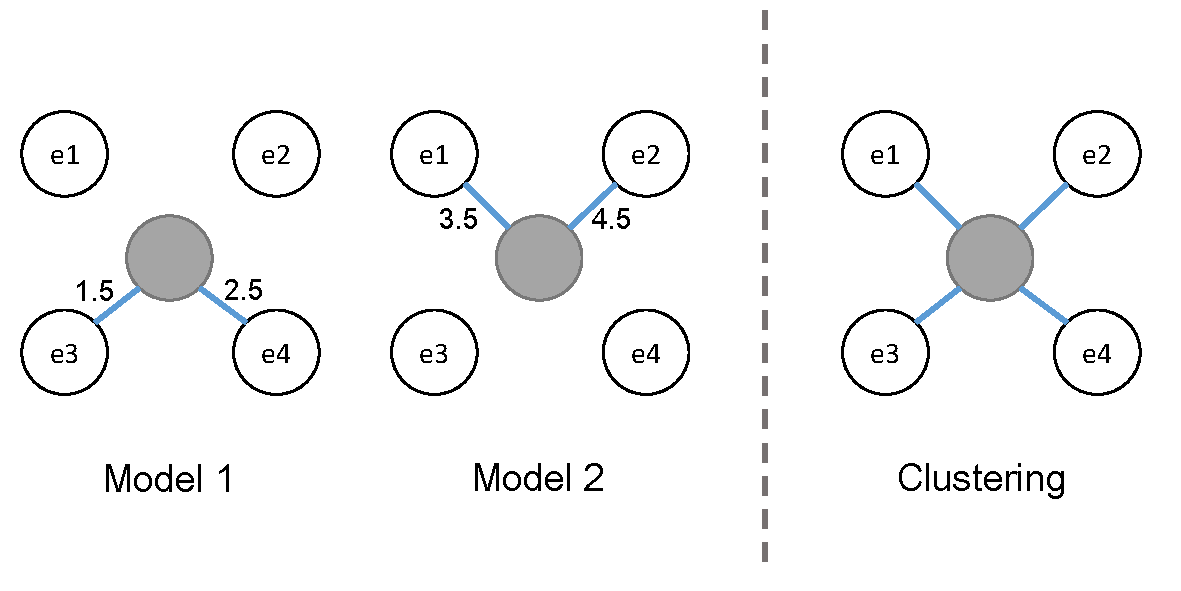
\includegraphics[width=0.4\textwidth]{./fig/lwe_d_graph}
\caption{An example of local neighborhood graphs of $x$ with distance into consideration.}
\label{graph_dist}
\end{figure}

\paragraph{Thresholding-based Adjustment}
The use of a \emph{weighted-average decision} for $x$ among base classifiers is reasonable when at least some classifiers perform well on $x$.
However, the similarity $s(G_{M_i}, G_C|x)$ for $M_i$ is expected to be small when the predictions of $M_i$ around $x$ conflict with its true local structure.
In such a case, using the decision from the classifier might not be a reasonable choice.
Since $s(G_{M_i}, G_C|x)$ reflects the consistency between classifier predictions and cluster structure, we use the average similarity score over all $M_i$ on $x$ as a discriminator to limit the usage of these base classifiers.
As an adjustment before the normalization of similarity scores, we check the average similarity score with,
\begin{equation}\label{ave_sim}
 \bar s_x = \frac {1}{k}\sum_{i=1}^k s(G_{M_i}, G_C|x)
\end{equation}
We continue with the ensemble prediction only if $\bar s_x$ is larger than a threshold $\delta$, and we will discuss the choice of $\delta$ in the evaluation section.


\subsubsection{Non-parametric Bayesian Clustering}
\label{sec_clustering}
In our transfer learning based approach, data density $p(x)$ is exploited via its latent clustering structure. We choose a Gaussian Mixture Model (GMM) \cite{zivkovic2004improved}, a partitional clustering algorithm, to perform the clustering.

In GMM, the cluster label for every instance is treated as a latent variable, which is drawn from a multinomial distribution $p(c)$, i.e., $p(c)\propto\alpha_c$, where $\forall c, \alpha_c\ge0$ and $\sum_c\alpha_c=1$. In any given cluster $c$, the conditional data likelihood of an instance $x$ is specified by a multivariate Gaussian distribution. To reduce the number of parameters to estimate, we choose the isotropic Gaussian in our solution,
\begin{equation}
p(x|c)=(2\pi\sigma^2)^{-d/2}\exp{-\frac{(x-\mu_c)^\mt (x-\mu_c)}{2\sigma^2}}
\end{equation}
where the variance $\sigma^2$ is shared by all the clusters. $\{\alpha_c, \mu_c\}^k_{c=1}$ and $\sigma$ are considered as model parameters in GMM.

However, in GMM, we need to manually specify the number of clusters for a given input data set; and the clustering result of GMM is very sensitive to this setting. More importantly,
in our study, usually there is more than one pattern in the point names even for the same type of sensors; therefore we cannot assume a class has only one cluster. It is impossible for us to predefine the
optimal cluster sizes. To make clustering feasible on the new building, we use a non-parameter Bayesian solution: we assume the model parameters $(\alpha, \mu)$ in each cluster are also random variables, which are drawn from a Dirichlet Process prior \cite{dp}.

A Dirichlet Process $DP(G_0, \eta)$ with a base distribution $G_0$ and a scaling parameter $\eta$ is a distribution over distributions~\cite{dp}. The base distribution $G_0$ specifies the prior distribution of model parameters, e.g., mean parameter $\mu$ in each cluster, and the scaling parameter $\eta$ specifies the concentration of samples drawn from the DP, e.g., cluster proportion $p(c)$. An important property of the DP is that though the draws from a DP have countably infinite size, they are discrete with probability one, which leads to a probability distribution on partitions of the data. The number of unique draws, i.e., the number of clusters, varies with respect to the data and therefore is random, instead of being pre-specified.

As a result, with the $DP(G_{0}, \eta)$ prior, the data density in a given collection of instances can be expressed using a stick-breaking representation
\cite{sethuraman1994constructive}:
\begin{equation}\label{eq_dp_density}
p(x)=\sum_{c=1}^\infty \alpha_c \mathcal{N}(x|\mu_c,\sigma)p(\mu_c|G_0)
\end{equation}
where $\alpha={\alpha}_{c=1}^\infty\sim Stick(\eta)$ represents the proportion of clusters in the whole collection. The stick-breaking process $Stick(\eta)$ for the cluster proportion parameter $\alpha$ is defined as: $\alpha'_c\sim Beta(1, \eta), \alpha_c=\alpha'_c\prod_{i=1}^{c-1}(1-\alpha'_i)$. Since the variance $\sigma^2$ is fixed in all clusters, we use a conjugate prior for $\mu$ in $G_0$, i.e., for $\forall c, \mu_{ci}\sim \mathcal{N}(a,b)$, with the assumption that each dimension in $\mu_c$ is independently drawn from a univariate Gaussian. This will greatly simplify the later on inference procedure.

Because the data density distribution defined in Eq~\eqref{eq_dp_density} only has finite support at the points of $\{\alpha_c, \mu_c\}^k_{c=1}$, we can calculate the posterior distribution of latent cluster labels in each unlabeled instance to discover the clustering structure. Following the sampling scheme proposed in \cite{neal2000markov}, we use a Gibbs sampling method to infer the posterior of cluster membership. Detailed specifications of this sampling algorithm can be found in \cite{neal2000markov}.


{\bf Putting it all together:} Algorithm~\ref{algo} summarizes our transfer learning algorithm for the sensor type classification across buildings.
We start by training a few base classifiers with the data features and labels of examples in a source building. We also generate clusters with DP on the name features of examples in the target building. For each example $x$ in the target building, we measure the local similarity score for each base classifier. If the average similarity is significant enough, we compute the weight for each classifier at $x$ by normalizing the similarity score. Finally we calculate the weighted sum of predictions from all base classifier and obtain the label $y$ for $x$.

\begin{algorithm}[ht]
 \caption{Transfer Learning for Sensor Type Classification}
 \label{algo}
 %\SetAlgoLined
 {\bf Input}: Data features of the source building $\mathcal{D_S}=\{x^D_1,x^D_2,\dots,x^D_n\}$ and their labels $\mathcal{Y_S}=\{y_1,y_2,\dots,y_n\}$  data features of the target building $\mathcal{D_T}=\{x^D_1,x^D_2,\dots,x^D_m\}$, and name features of the target building $\mathcal{P_T}=\{x^P_1,x^P_2,\dots,x^P_m\}$\\
 {\bf Output}: predicted labels of the examples in target building $\mathcal{Y}$\\
 Initialize: Generate clusters with $DP(G_{0}, \eta)$ on $\mathcal{P_T}$\\
 Train $k$ classifiers $M_1, \dots, M_k$ based on $\mathcal{D_S}$ and $\mathcal{Y_S}$\;

\For{$x^D$ in $\mathcal{D_T}$}{
Construct neighborhood graphs $G_M$ and $G_C$ for $x^D$ as defined in Section~\ref{sec:gwe} for each $M_i$;\\
Compute the similarity score for each $M_i$ with Eq.~\ref{d_sim};\\
Check the average similarity score $\hat s_x$ over all $M_i$ with Eq.~\ref{ave_sim};\\
If $\hat s_x > \delta$, then use Eq.~\ref{eq_norm} and Eq.~\ref{eq_sum} to predict the label $y$;
}
\end{algorithm}
